\graphicspath{{Baroclinic_mode/code/figs/}}

We solve the baroclinic mode for arbitrary stratification profiles. That is, we solve the Sturm–Liouville problem:
\begin{align}
&\frac{\mathrm{d}}{\mathrm{d}z}\left( \frac{f^2}{N^2}\frac{\mathrm{d}\psi}{\mathrm{d}z} \right) = -\lambda^2\psi\\
\text{with}\qquad &\frac{\mathrm{d}\psi}{\mathrm{d}z}(z=0)=\frac{\mathrm{d}\psi}{\mathrm{d}z}(z=-H)=0
\end{align}
where $N^2$ is a function of $z$.

We pose the problem on $H\in[-1,0]$ with $f^2/N^2(z)=e^{z}$. Realistic physical values only change the eigenvalues by a constant. We use the eigenvalue problem module of Dedalus. The eigenvalues and eigenvectors (the baroclinic mode) are shown in Figure \ref{fig:expo_bc_mode}.

\begin{figure}
    \centering
    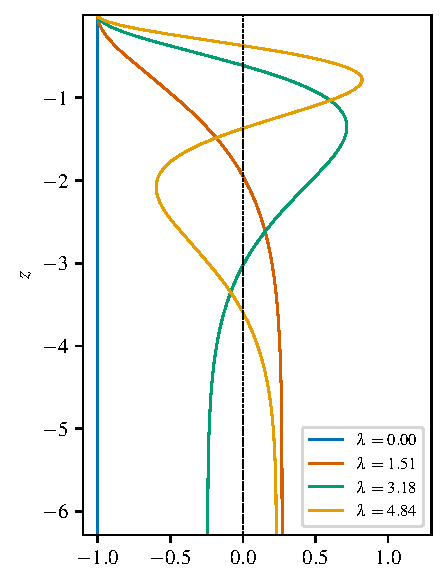
\includegraphics{expo_bc_mode}
    \caption{}
    \label{fig:expo_bc_mode}
\end{figure}

There are many definitions of orthogonal vertical mode for the ocean. For some examples, see \cite{SmithVanneste_13,LaCasce_17,YassinGriffies_22}. All these problems can be solved by Dedalus, with more or less modification of the above code. One could also input realistic stratification profiles from data, interpolating them onto a Chebyshev grid of sufficient resolution. In particular, this code reproduces the functionality of \url{https://github.com/rabernat/oceanmodes}. 